\documentclass[../main.tex]{subfiles}

\graphicspath{{\subfix{../imgs/}}}

\begin{document}

\section{Virtuoso and the Analog Workflow}

\subsection{Nanometer Design Challenges}

\subsection{The $g_m$/$I_D$ Method}

Many mainstream methods for sizing generally assume strong inversion and use the overdrive voltage $V_{OD}$ at a key parameter. For nanometer, low-power design this proves a limitation. In this section, we will introduce the $g_m/I_D$ method, which allows us to exploit weak inversion models and the subthreshold region. The method proves reliable and has several advantages. \vspace*{10pt}

The method is based on the transconductance over DC drain current ratio($g_m/I_D$ versus the normalized drain current $I_N = I_D/(W/L)$. The ratio $g_m/I_D$ is effectively a measure of the efficiency to translate current (and therefore power) into $g_m$ (which in turn means gain). The $g_m/I_D$ curve can be observed as the derivative of $I_D$ with respect to $V_{GS}$

$$ 
\frac{g_m}{I_D} = \frac{1}{I_D} \cdot \frac{\partial I_D}{\partial V_{GS}} = \frac{\partial (\ln I_D)}{\partial V_{GS}}
$$

\noindent
In the weak inversion region, the derivative is maximum due to the exponential dependence of $I_D$ in relation to $V_{GS}$.

\pagebreak

\subsection{Reference Curves}

The $g_m/I_D$ depends entirely on the accuracy of the MOS models from the PDK. We plot three reference curves which will then allows us to size all transtors accurately and fast.

\begin{figure}[H]
    \centering
    \begin{subfigure}{0.5\textwidth}
      \centering
      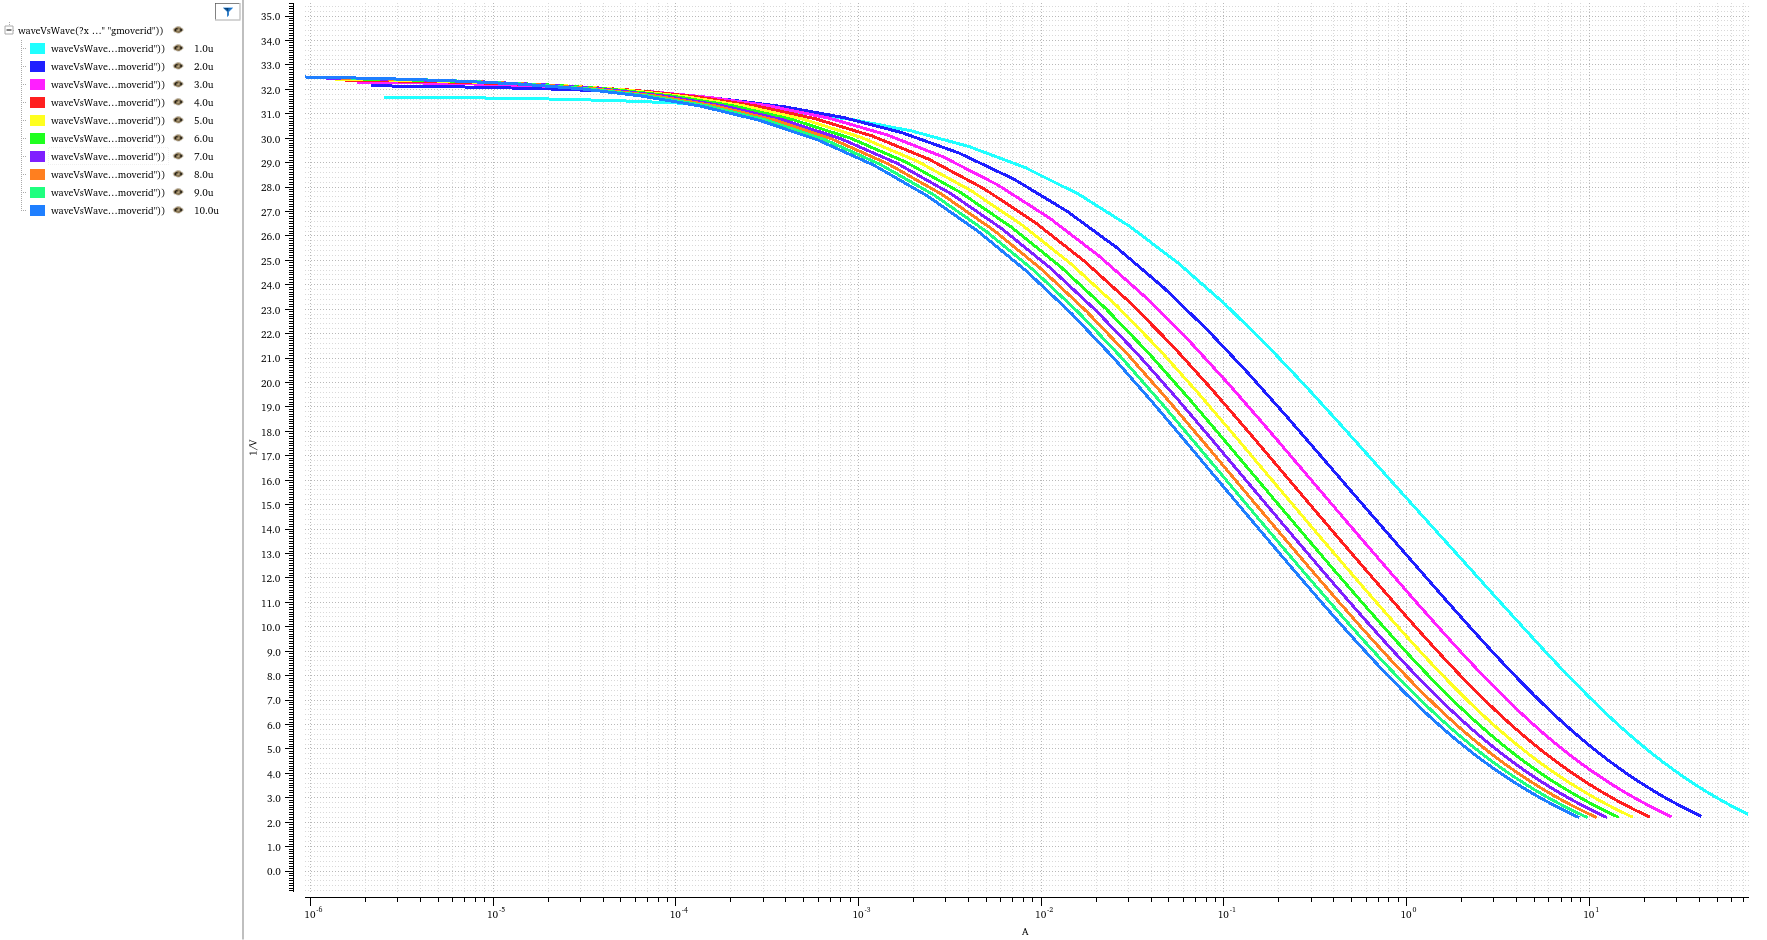
\includegraphics[width=.9\textwidth]{nmos-gm-idw-coarse-inv.png}
      \caption{NMOS}
    \end{subfigure}%
    \begin{subfigure}{0.5\textwidth}
      \centering
      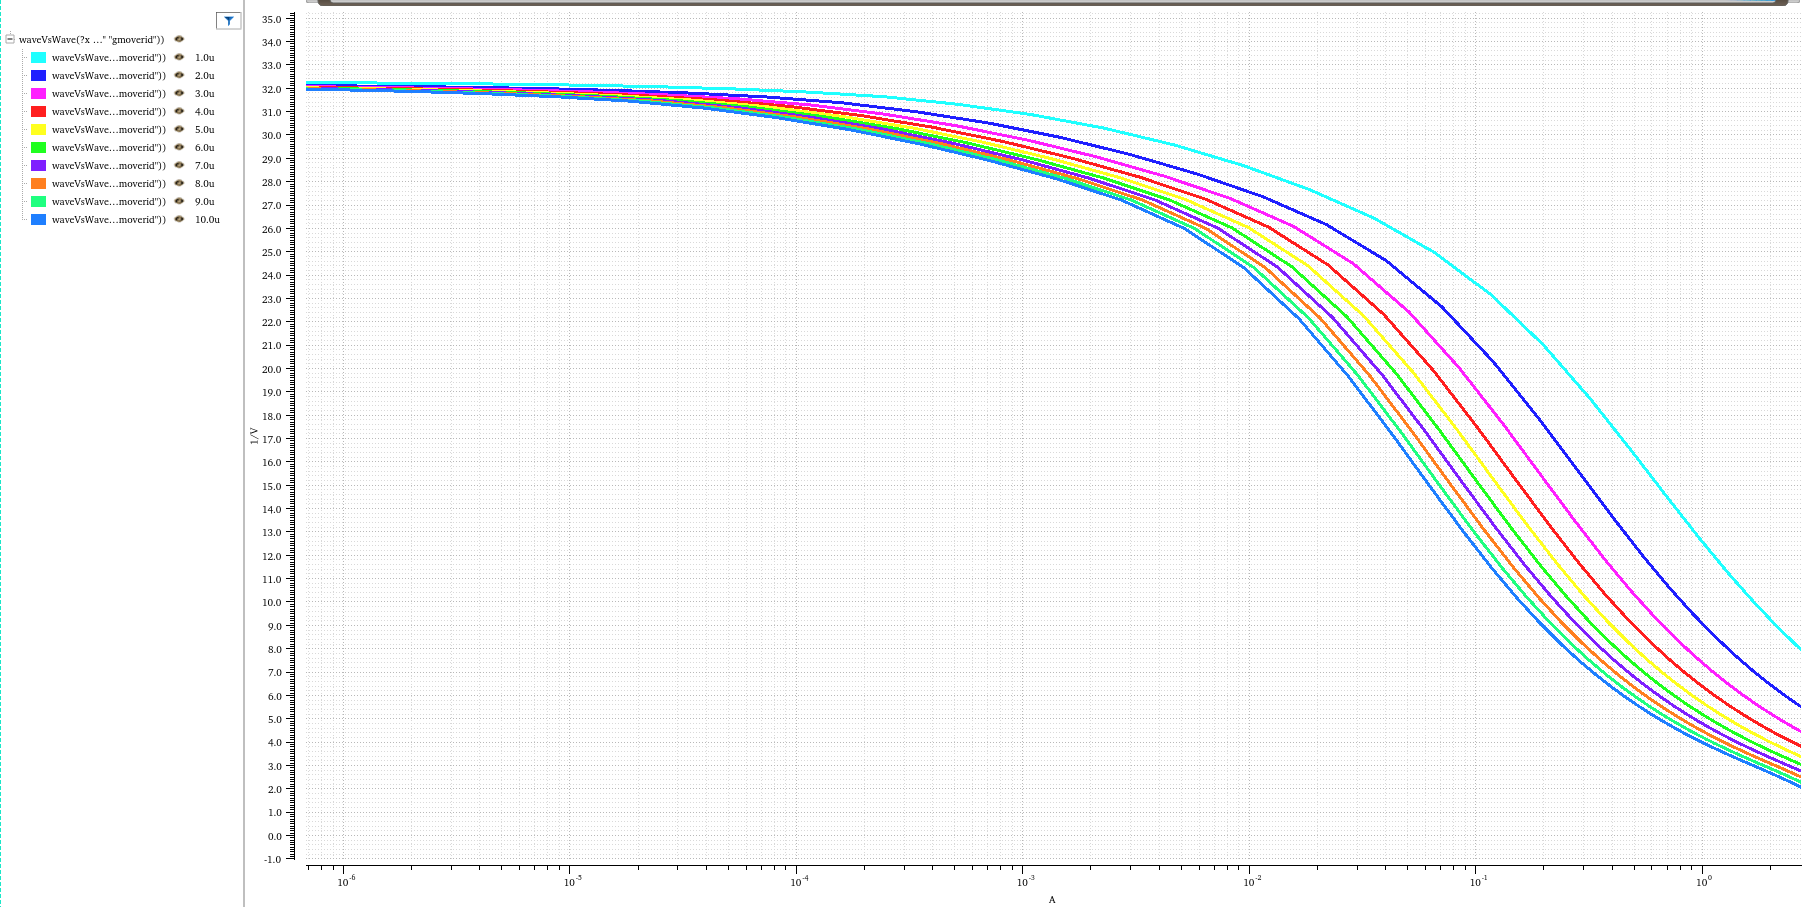
\includegraphics[width=.9\textwidth]{pmos-gm-idw-coarse-inv.png}
      \caption{PMOS}
    \end{subfigure}
    \caption{$g_m/I_D$ versus normalized drain current $I_N$}
\end{figure}

\begin{figure}[H]
    \centering
    \begin{subfigure}{0.5\textwidth}
      \centering
      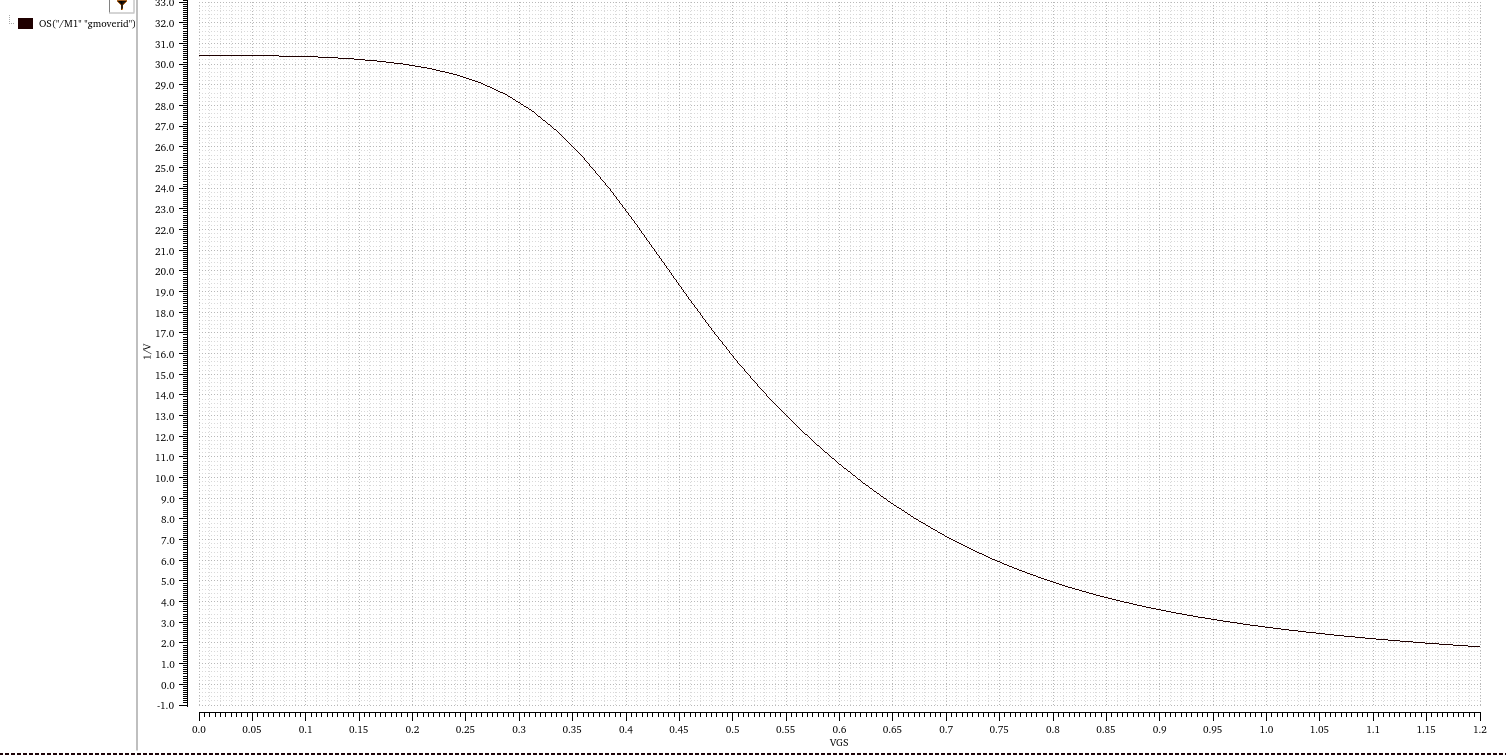
\includegraphics[width=.9\textwidth]{nmos-gm-id-vgs-inv.png}
      \caption{NMOS}
    \end{subfigure}%
    \begin{subfigure}{0.5\textwidth}
      \centering
      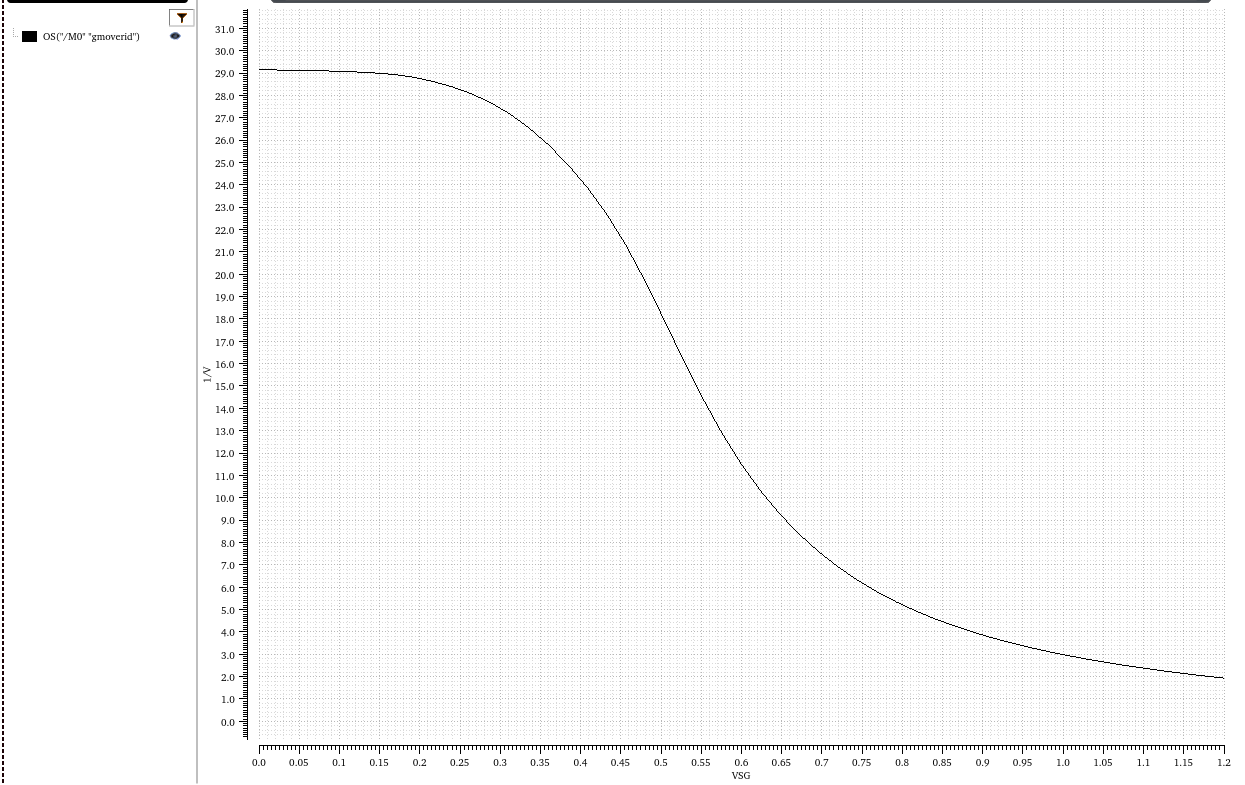
\includegraphics[width=.9\textwidth]{pmos-gm-id-vgs-inv.png}
      \caption{PMOS}
    \end{subfigure}
    \caption{$g_m/I_D$ versus $V_{GS}$}
\end{figure}

\begin{figure}[H]
    \centering
    \begin{subfigure}{0.5\textwidth}
      \centering
      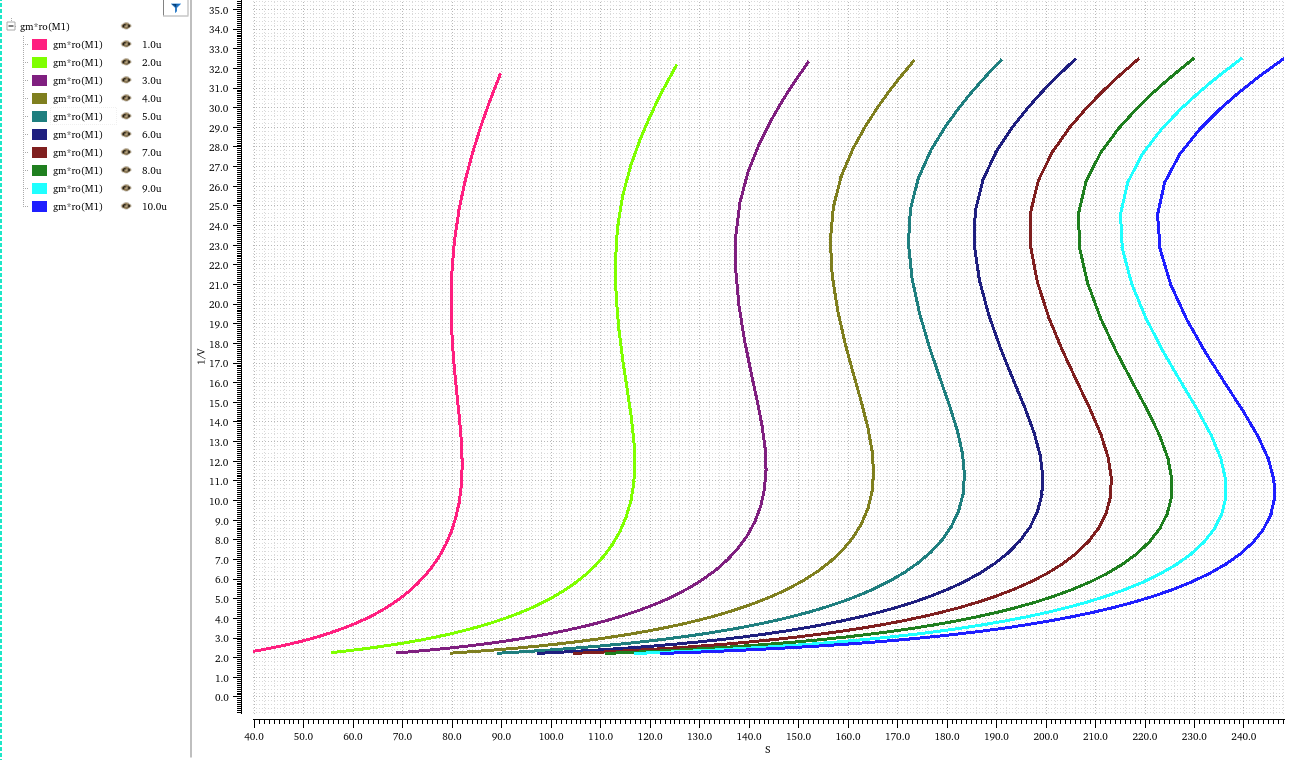
\includegraphics[width=.9\textwidth]{nmos-gm-id-gmro-inv.png}
      \caption{NMOS}
    \end{subfigure}%
    \begin{subfigure}{0.5\textwidth}
      \centering
      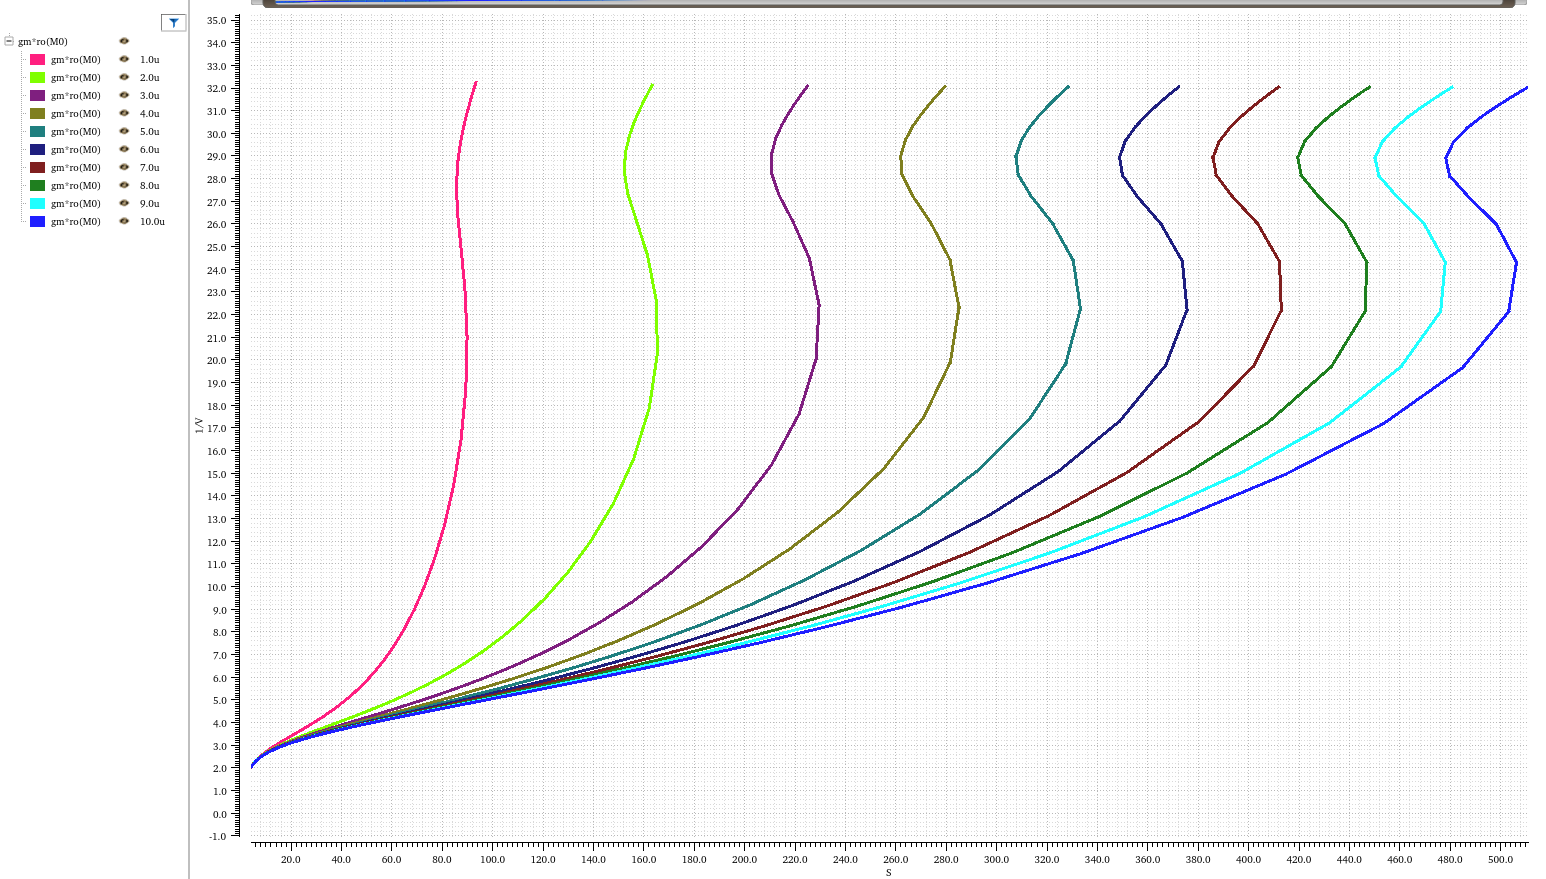
\includegraphics[width=.9\textwidth]{pmos-gm-id-gmro-inv.png}
      \caption{PMOS}
    \end{subfigure}
    \caption{$g_m/I_D$ versus $g_m r_O$}
\end{figure}

\pagebreak






\end{document}